\chapter{Algorithm: Nearest sample matting}
\label{chap:nearest-sample-matting}

%\section{Introduction}
%\label{sec:introduction}

After reviewing various matting methods we noticed that each algorithm works best in specific cases and algorithms that work for all cases do not give satisfying results. The steps that formulate an algorithm that are common in all matting methods consist of getting the input data to be segmented either as an image or as a video frame, get the prior information either by user input or automatically using the methods described in Chapter 2, sample foreground and background pixels based on the prior information to create a training set of data that characterises the image background and foreground, and then select the best foreground and background samples in order to classify each unknown pixel into those two sets definitely or relatively based the matting equation so that an alpha matte is created. The last step is to refine the estimated alpha matte for smoothness. 

\begin{algorithm}
\caption{Matting methodology}\label{matting-method}
\begin{algorithmic}[1]
\State Get input image
\State Get trimap
\ForAll{unknown pixels}
\State Sample F and B
\State Get best F and B
\State Calculate $\alpha$
\EndFor
\State Refine alpha matte
\end{algorithmic}
\end{algorithm}

For the formulation of our own algorithm we considered the steps mentioned above and focused on getting an accurate matte using benchmark datasets and images produced by the Kinect sensor, without using refinement methods for smoothness or connectivity.

%%%%%%%%%%%%%%%%%%%%%%%%%%%%%%%%%%%%%%%%%%%%%%%%%%%%%%%%%%%%%%%%%%%%
\section{Sampling}
\label{sec:sampling}

The sampling procedure starts by iterating through each unknown pixel and for each one all the neighbouring pixels that belong to foreground and background are sampled within a small radius. The sampling radius around the unknown pixel grows until a specified amount of samples is gathered. This methodology samples the most spatially close pixels and according to other matting methods, pixels that are close to each other tend to share similar attributes and thus increase the probability of correct classification. For scribble based trimaps we used a global sampling approach, where all pixels in the definite foreground and definite background are used as samples. When using global sampling and the number of samples is too high, experiments on images with small fuzzy regions showed that sampling every other or every few pixels (50\%-20\% of total) reduces running time significantly with little affect on the resulting alpha matte quality .This again, is due to the fact that pixels that are close share similar attributes.

\begin{algorithm}
\caption{Sampling algorithm}\label{sampling-algorithm}
\begin{algorithmic}[1]
\ForAll{unknown pixels}
\While{$F\; set < min\; \textbf{OR}\; B\; set < min$}
\ForAll{pixels in radius R}
\State Add pixel to \textit{F set}
\State Add pixel to \textit{B set}
\EndFor
\State R $\gets$ R + 1
\EndWhile
\State Classification
\EndFor
\end{algorithmic}
\end{algorithm}

\begin{figure}[t!]
\centering
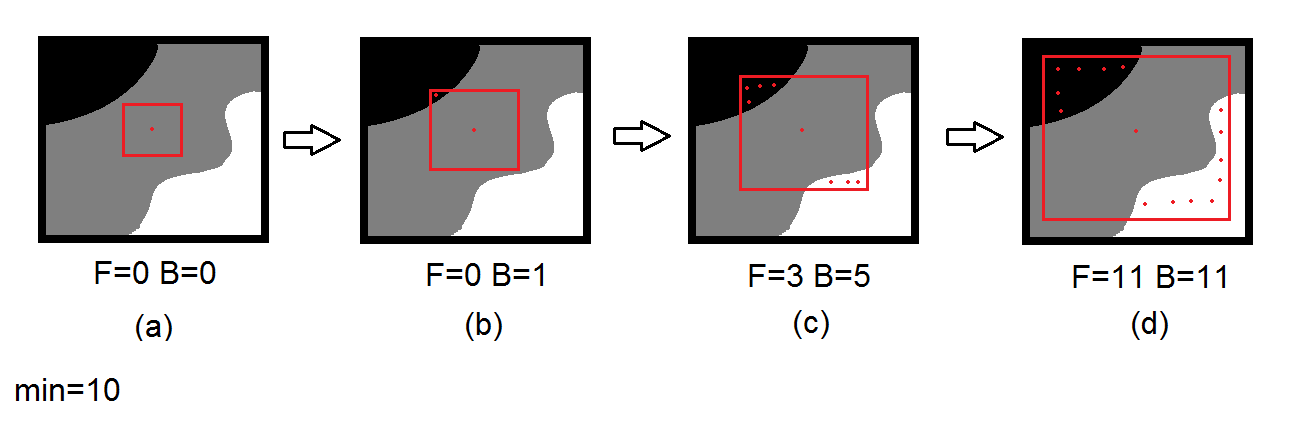
\includegraphics[width=1\columnwidth]{Chapter5/5/win.png}
\caption[Sampling radius.]{The sampling radius grows until a minimun number of F and B samples is gathered.}
\label{fig:window-f}
\end{figure}

\begin{figure}[t!]
\centering
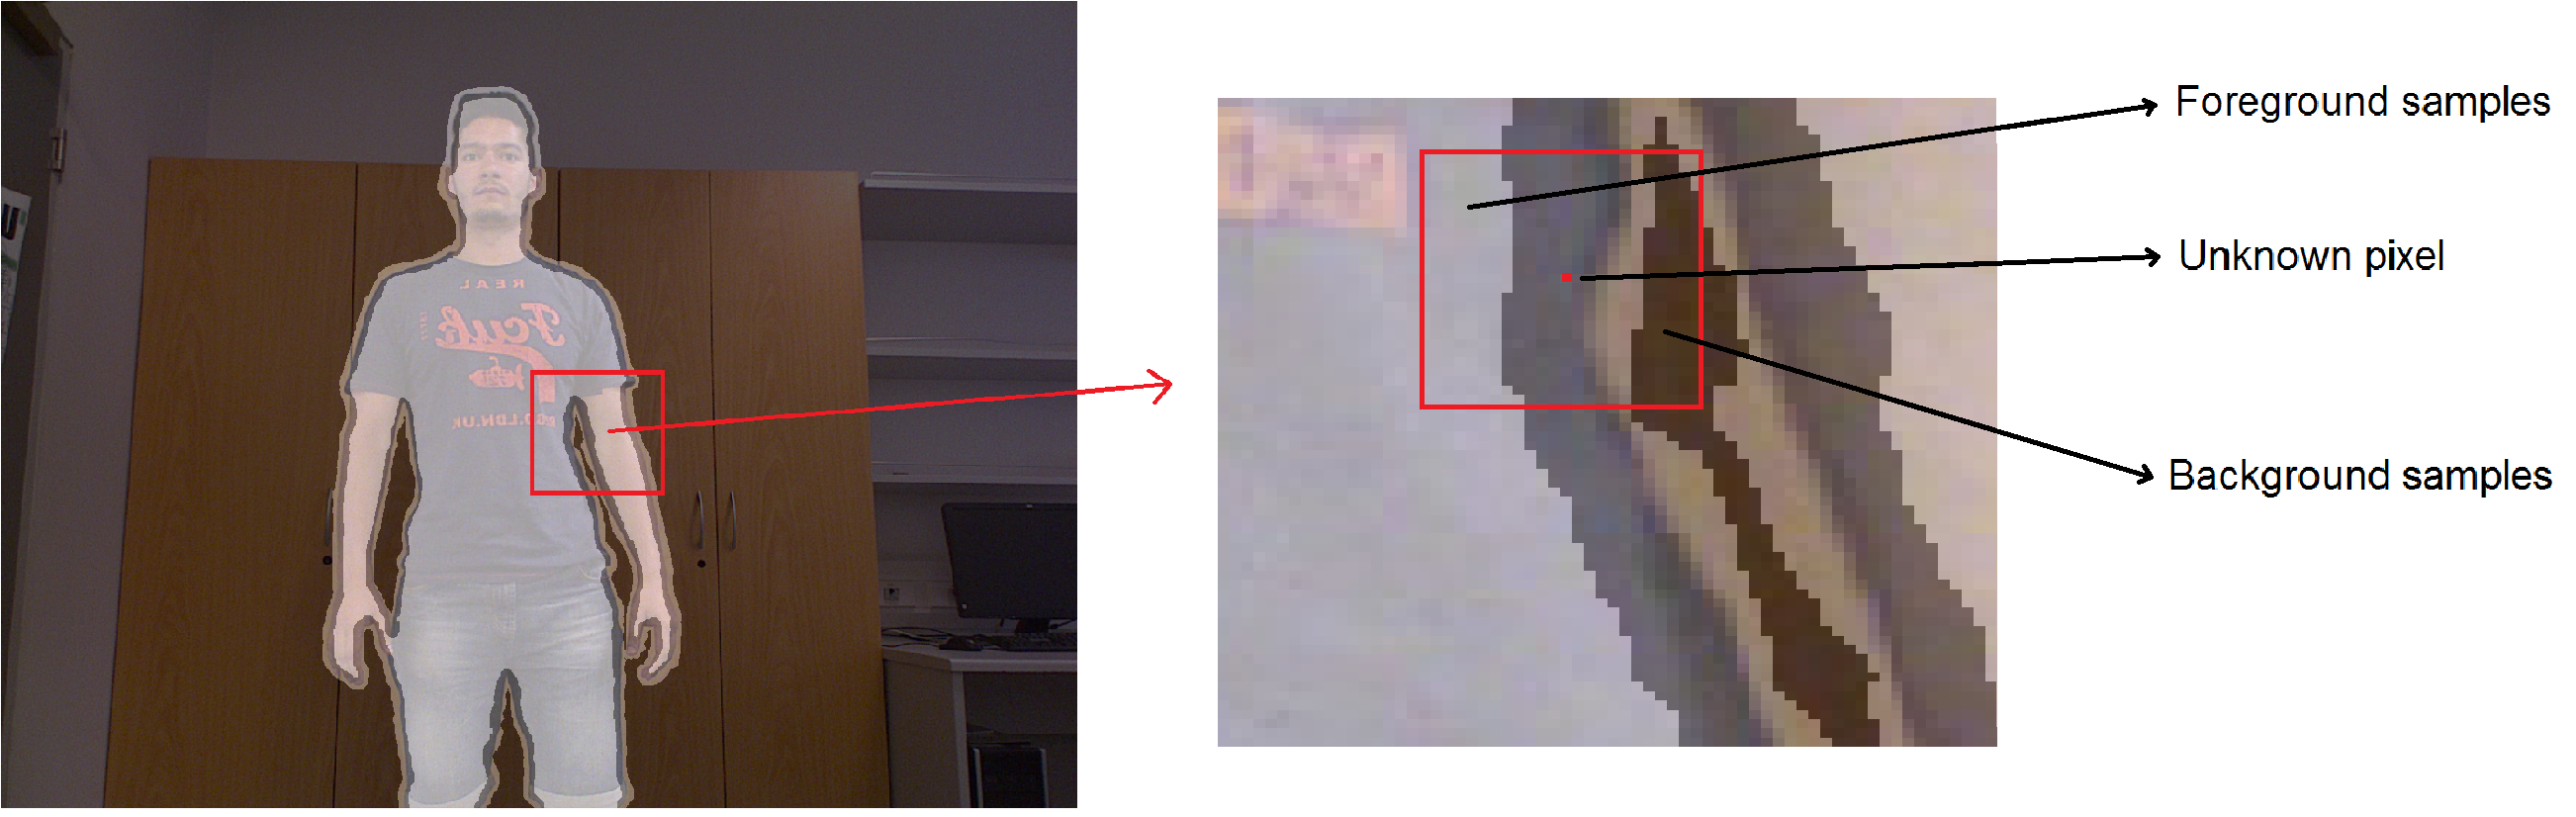
\includegraphics[width=1\columnwidth]{Chapter5/5/sampling_window.jpg}
\caption[New sampling strategy.]{Sampling strategy that gathers all the pixels within a window around an unknown pixel.}
\label{fig:sampling-window-f}
\end{figure}

%%%%%%%%%%%%%%%%%%%%%%%%%%%%%%%%%%%%%%%%%%%%%%%%%%%%%%%%%%%%%%%%%%%%%
\section{Classification}
\label{sec:classification}

For each sample a feature vector is created that contains colour space and spatial information. Then each sample from the foreground and background sample sets are compared with the unknown using the Euclidean distance (\ref{eq:ours_e1}) as a metric and the foreground and background samples with minimum distance are considered the best samples to be used for alpha estimation (\ref{eq:ours_e2}).

\begin{equation} \label{eq:ours_e1}
E(V_{c},V_{s})=\sqrt{\sum_{i=1}^{S}(V_{c_i}-V_{s_i})^{2}}
\end{equation}

\begin{equation} \label{eq:ours_e2}
[F,B]=argmin\sum _{i\epsilon S}E(V_c,V_s)_{i}
\end{equation}

The features used to characterize a pixel can vary; different colour spaces can be used and spatial information can be omitted depending on the scenario. The alpha value for the unknown pixel is computed by substituting the selected \textit{F} and \textit{B} samples in (\ref{eq:ours_e3}), which is a rearranged version of the matting equation. 

\begin{equation} \label{eq:ours_e3}
\alpha=\frac{(C-B)(F-B)}{\left \| F-B \right \|^{2}}
\end{equation}

\begin{algorithm}
\caption{Classification algorithm}\label{classification-algorithm}
\begin{algorithmic}[1]
\ForAll{unknown pixels}
\State Sampling
\ForAll{pixels in F set}
\State distance $\gets$ Eucledian(Foreground, Unknown)
\If{$distance < min$}
\State best Foreground $\gets$ Foreground
\State min $\gets$ distance
\EndIf
\EndFor
\ForAll{pixels in B set}
\State distance $\gets$ Eucledian(Background, Unknown)
\If{$distance < min$}
\State best Background $\gets$ Background
\State min $\gets$ distance
\EndIf
\EndFor
\State $\alpha$ $\gets$ estimate\;alpha(best Foreground, best Background)
\EndFor
\end{algorithmic}
\end{algorithm}

%%%%%%%%%%%%%%%%%%%%%%%%%%%%%%%%%%%%%%%%%%%%%%%%%%%%%%%%%%%%%%%%%%%%%%%
\section{Results and comparisons}
\label{sec:results-and-comparisons}

For experiments and resulting alpha matte comparisons, benchmark datasets from \cite{benchmark} where used along with images taken from the Kinect sensors.
The methodology was tested using trimaps with wide and narrow unknown regions and with scribble based trimaps. Also the number of samples and the features used for classification and in order to see how these parameters affect the results.
For comparison, results from other matting methods were taken from \cite{benchmark}.
\par
In Figure \ref{fig:troll-f} the troll image is part of the test images from the benchmark dataset, and is considered an image with moderate transparency and difficult background. The hair is the major point of interest because most of it is within the unknown region and part of it has a background with similar colours. The Bayesian approach (Figure \ref{fig:troll-f}c) produces many erroneous $\alpha$ values and has practically no smoothness in the hair region. Closed-Form matting produces a smooth alpha matte but includes whole regions of the background into the alpha matte (Figure \ref{fig:troll-f}d). Our resulting alpha matte has moderate smoothness and manages to classify correctly most of the background pixels that are ambiguous (Figure \ref{fig:troll-f}e). By using the HSV colour space and omitting spatial information, more background pixels are removed but low opacity foreground pixels are also lost (Figure \ref{fig:troll-f}f).

\begin{figure}[t!]
%\centering
\subfloat[][RGB image]{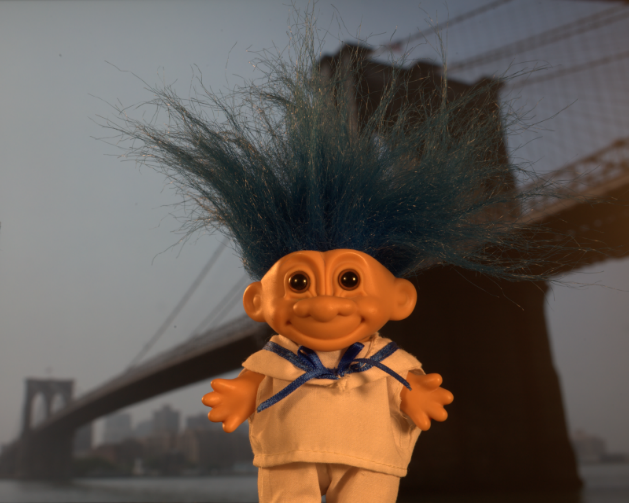
\includegraphics[width=0.5\columnwidth]{Chapter5/5/troll_color.png}}
\subfloat[][Trimap]{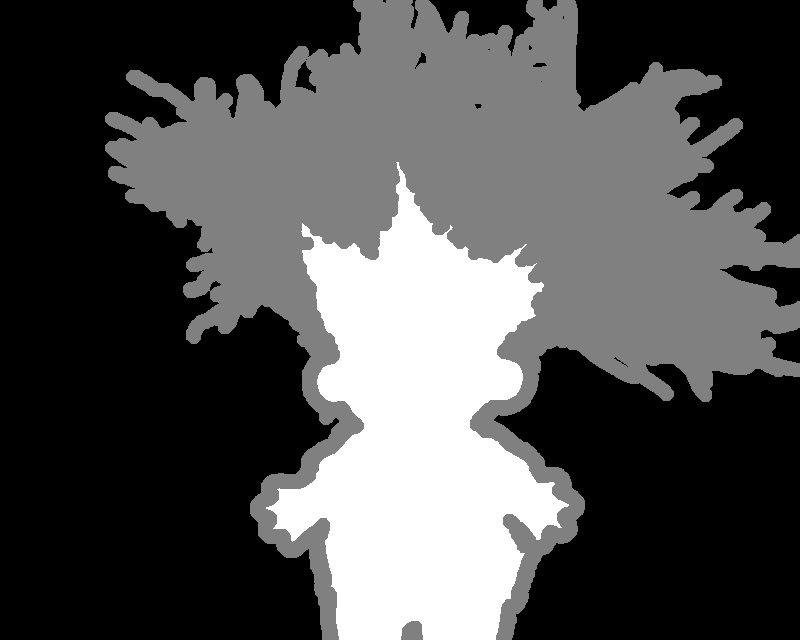
\includegraphics[width=0.5\columnwidth]{Chapter5/5/troll_trimap.png}}
\newline
\subfloat[][Bayesian result]{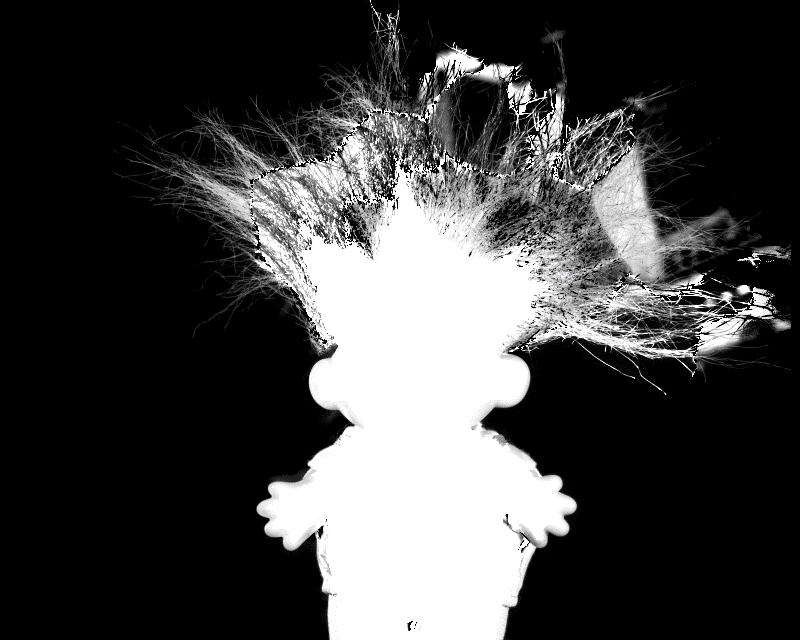
\includegraphics[width=0.5\columnwidth]{Chapter5/5/troll_bayesian.png}}
\subfloat[][Closed-form result]{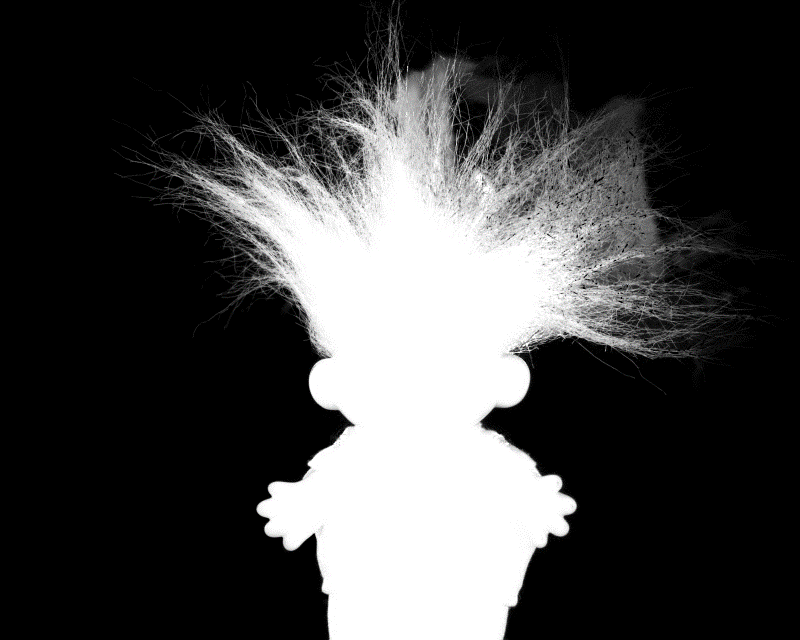
\includegraphics[width=0.5\columnwidth]{Chapter5/5/troll_closed_form.png}}
\newline
\subfloat[][HSV and spacial]{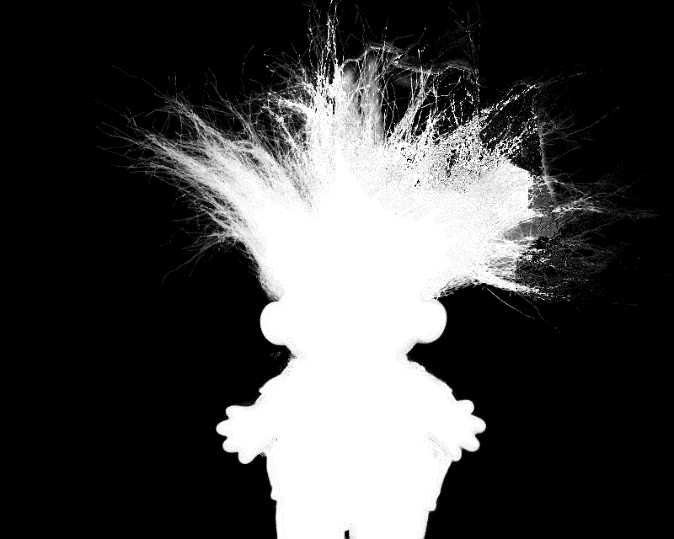
\includegraphics[width=0.5\columnwidth]{Chapter5/5/troll_hsvij.png}}
\subfloat[][HSV only]{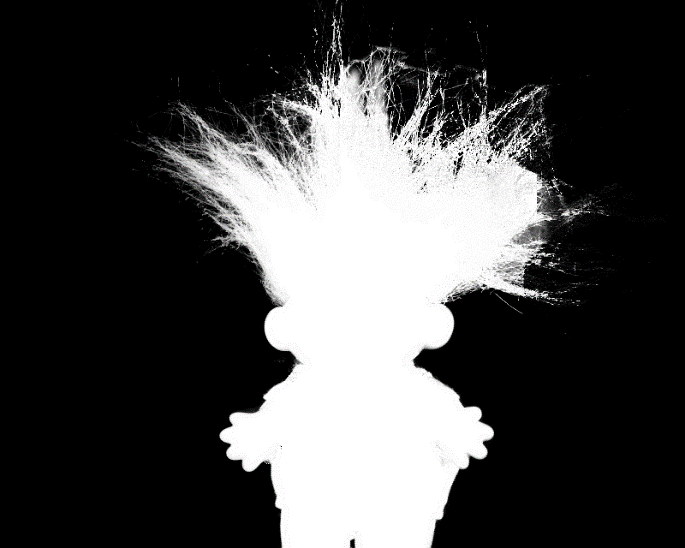
\includegraphics[width=0.5\columnwidth]{Chapter5/5/troll_hsv.png}}
\caption[Troll benchmark image with various results.]{Troll image with results from Bayesian, Closed-Form and ours, using HSV colour space and local sampling.}
\label{fig:troll-f}
\end{figure}

The next result is another test benchmark image (Figure \ref{fig:donkey-f}) that identically to the previous result, has moderate transparency and some ambiguous regions. Regions with hair are misclassified when the background has similar colours; in the Bayesian by excluding many pixels (Figure \ref{fig:donkey-f}c) and in Closed-Form by adding extra background regions in an attempt to smooth the alpha matte (Figure \ref{fig:donkey-f}d). Our method manages to capture most of the hair, but still omits foreground pixels that have similar colours to the background even when spatial information is used (Figure \ref{fig:donkey-f}e).

\begin{figure}[t!]
%\centering
\subfloat[][RGB image]{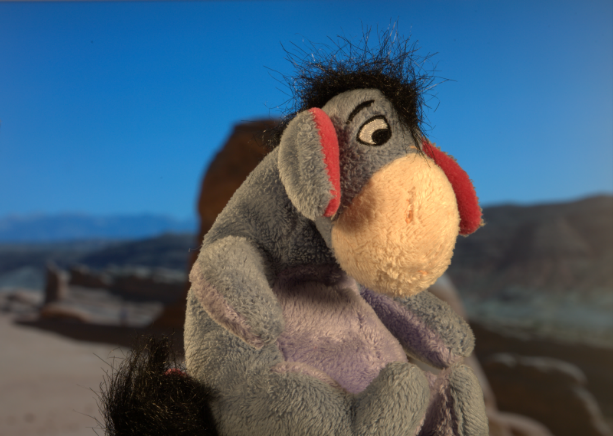
\includegraphics[width=0.5\columnwidth]{Chapter5/5/donkey_color.png}}
\subfloat[][Trimap]{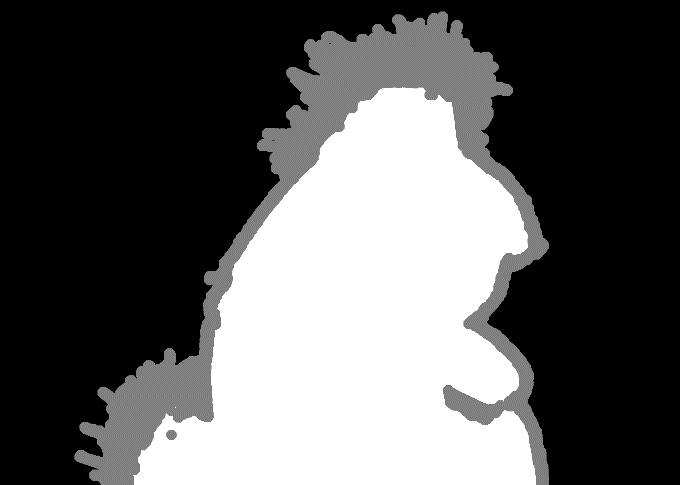
\includegraphics[width=0.5\columnwidth]{Chapter5/5/donkey_trimap.png}}
\newline
\subfloat[][Bayesian result]{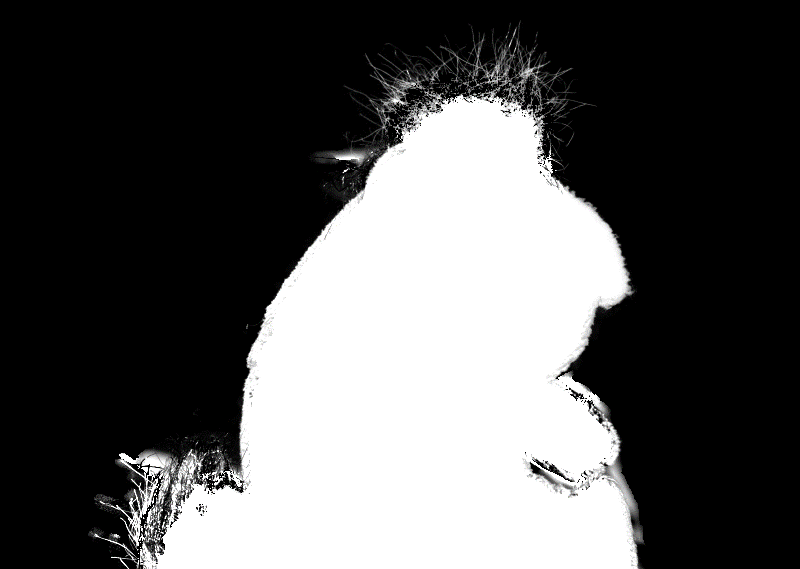
\includegraphics[width=0.5\columnwidth]{Chapter5/5/donkey_bayesian.png}}
\subfloat[][Closed-form result]{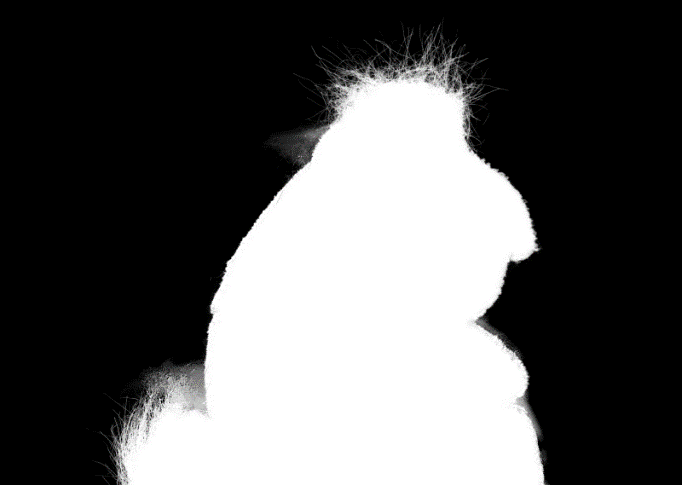
\includegraphics[width=0.5\columnwidth]{Chapter5/5/donkey_closed_form.png}}
\newline
\subfloat[][HSV and spacial]{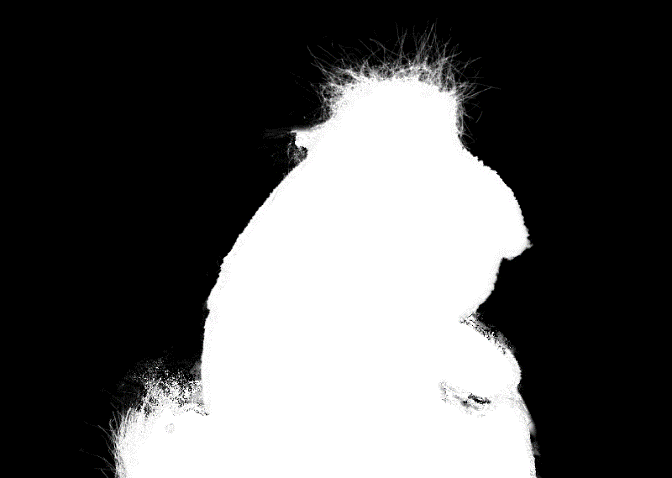
\includegraphics[width=0.5\columnwidth]{Chapter5/5/donkey_hsvij.png}}
\subfloat[][HSV only]{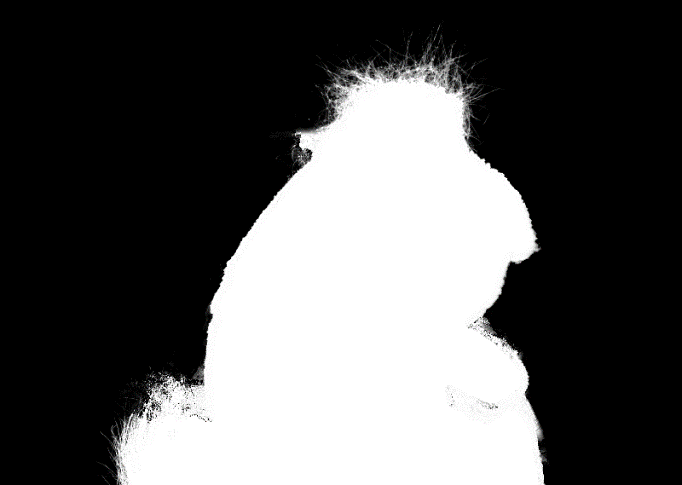
\includegraphics[width=0.5\columnwidth]{Chapter5/5/donkey_hsv.png}}
\caption[Donkey benchmark image with various results.]{Donkey image with results from Bayesian, Closed-Form and ours, using HSV colour space and local sampling.}
\label{fig:donkey-f}
\end{figure}

The next result presented is from \cite{closedform}, and is using a scribble based trimap for a high opacity image (Figure \ref{fig:peacock-f}). In this case, instead of sampling locally, since prior information is limited, all the pixels in definite F and B are used. The Closed-Form result is almost 100\% accurate visually and is presented in as part of their experimental results in \cite{closedform} (Figure \ref{fig:peacock-f}c). When using colour and spatial information our result is quite close to Closed-Form but some artifacts exists in the background (Figure \ref{fig:peacock-f}d) due to the facts that our method does not refine the alpha matte or consider smoothness. By using only colour values for classification the artifacts are removed but many low opacity pixels are lost (Figure \ref{fig:peacock-f}e).

\begin{figure}[t!]
%\centering
\subfloat[][RGB image]{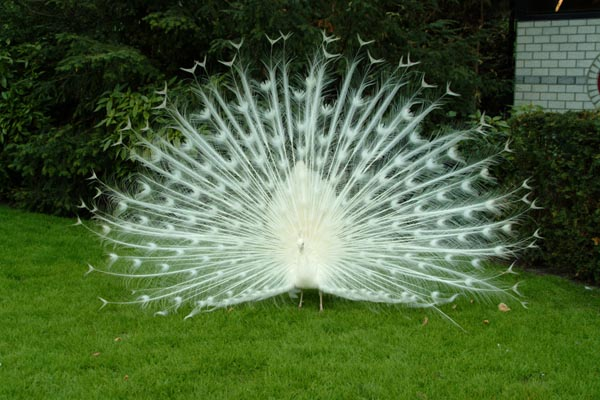
\includegraphics[width=0.5\columnwidth]{Chapter5/5/peacock_color.png}}
\subfloat[][Trimap]{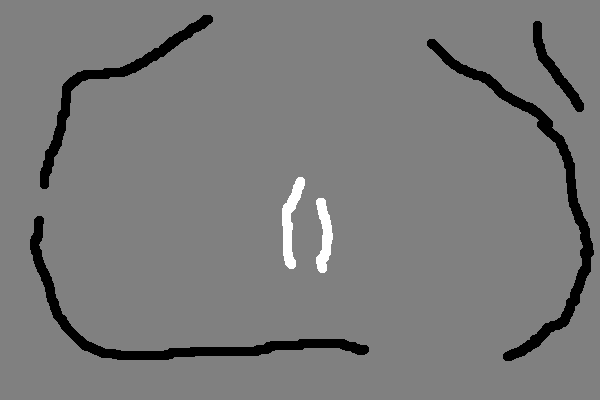
\includegraphics[width=0.5\columnwidth]{Chapter5/5/peacock_trimap.png}}
\newline
\subfloat[][Closed-form result]{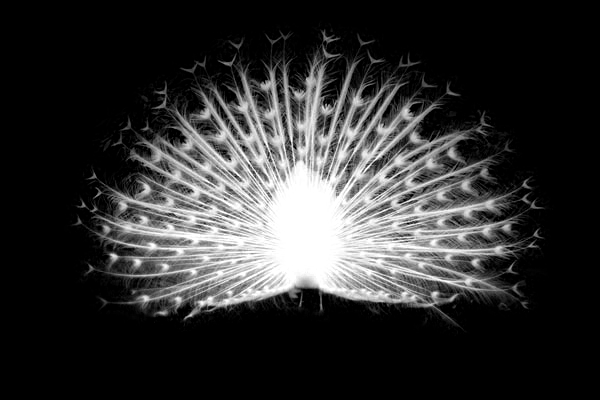
\includegraphics[width=0.5\columnwidth]{Chapter5/5/peacock_closed_form.png}}
\newline
\subfloat[][RGB and spacial]{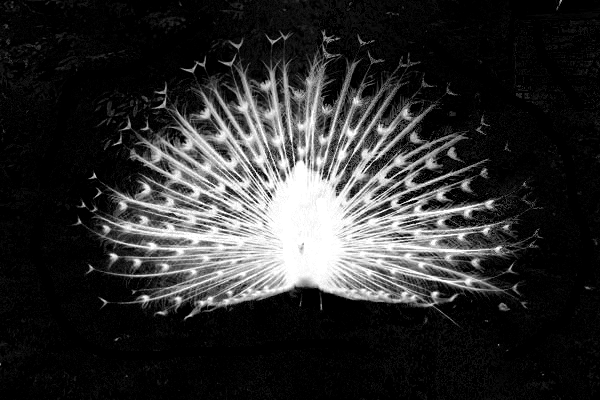
\includegraphics[width=0.5\columnwidth]{Chapter5/5/peacock_rgbij.png}}
\subfloat[][RGB only]{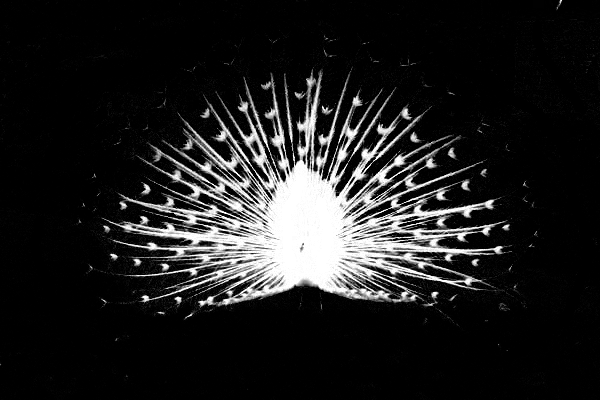
\includegraphics[width=0.5\columnwidth]{Chapter5/5/peacock_rgb.png}}
\caption[Peacock benchmark image with various results.]{Peacock image with results from Closed-Form and ours, using global sampling.}
\label{fig:peacock-f}
\end{figure}

The next figures display results of images from the training benchmark dataset and our results are compared with the ground truth. For a moderate opacity image (Figure \ref{fig:trolls-f}a) very few errors are visible (Figure \ref{fig:trolls-f}d), mainly in regions where colours are similar. In Figure \ref{fig:bear-f}a the background is easy to distinguish and the result is practically 100\% accurate (Figure \ref{fig:bear-f}d).

\begin{figure}[t!]
\centering
\subfloat[][RGB image]{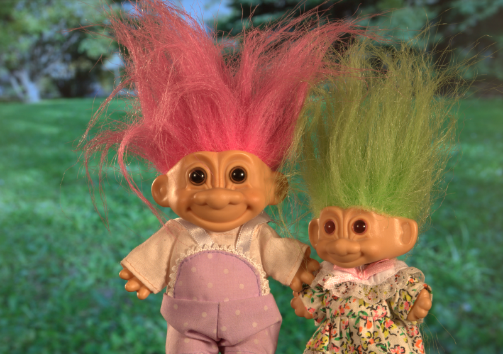
\includegraphics[width=0.4\columnwidth]{Chapter5/5/trolls_color.png}}
\subfloat[][Trimap]{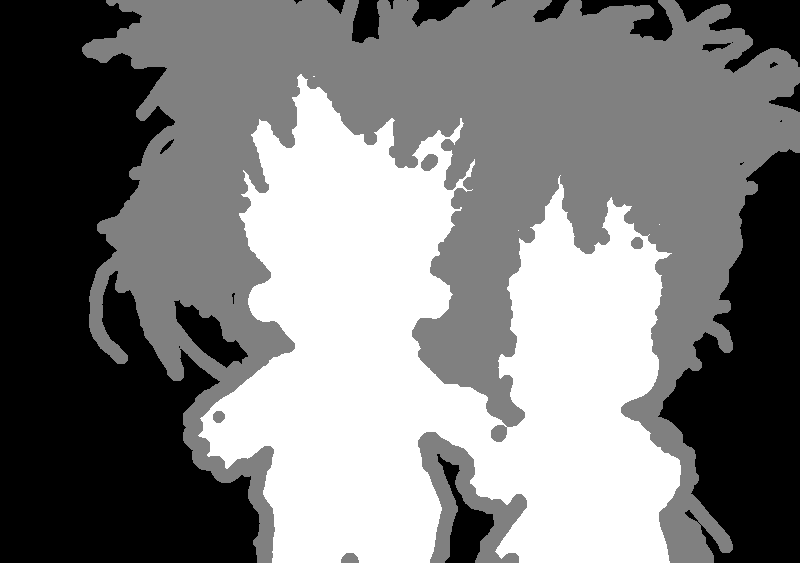
\includegraphics[width=0.4\columnwidth]{Chapter5/5/trolls_trimap.png}}
\newline
\subfloat[][Ground truth]{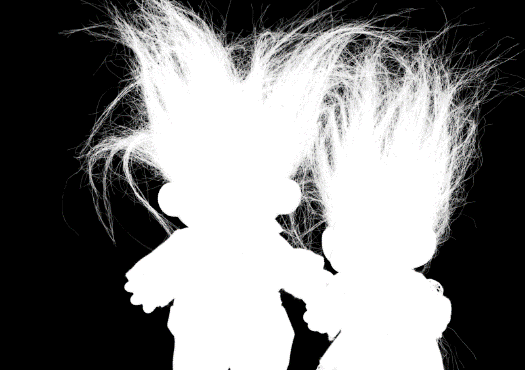
\includegraphics[width=0.4\columnwidth]{Chapter5/5/trolls_gt.png}}
\subfloat[][Our result]{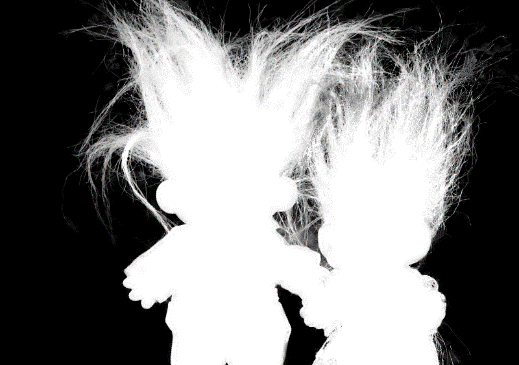
\includegraphics[width=0.4\columnwidth]{Chapter5/5/trolls_ours.png}}
\caption[GT04 benchmark image with various results.]{GT04 ground truth in comparison with our result.}
\label{fig:trolls-f}
\end{figure}

\begin{figure}[t!]
\centering
\subfloat[][RGB image]{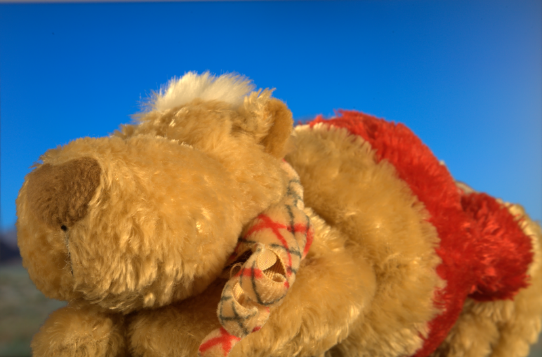
\includegraphics[width=0.4\columnwidth]{Chapter5/5/bear_color.png}}
\subfloat[][Trimap]{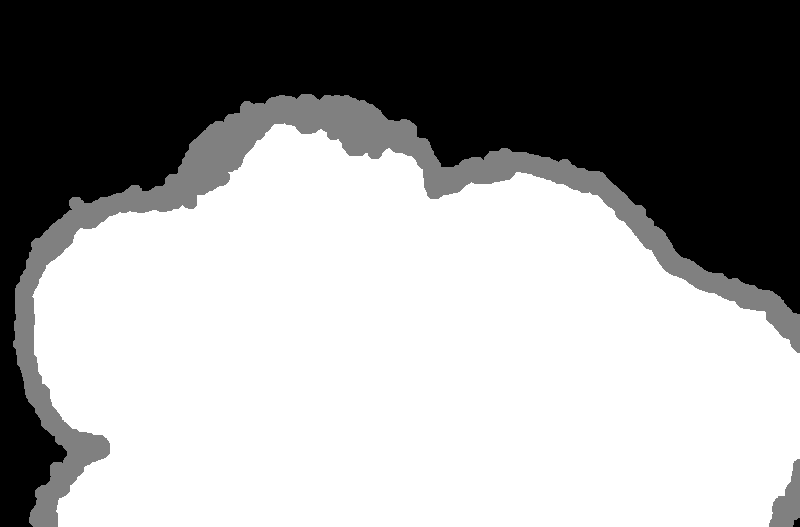
\includegraphics[width=0.4\columnwidth]{Chapter5/5/bear_trimap.png}}
\newline
\subfloat[][Ground truth]{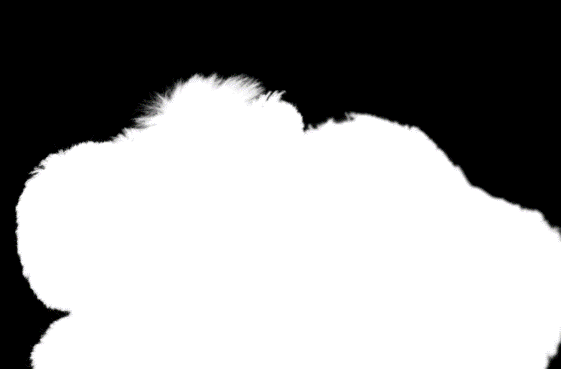
\includegraphics[width=0.4\columnwidth]{Chapter5/5/bear_gt.png}}
\subfloat[][Our result]{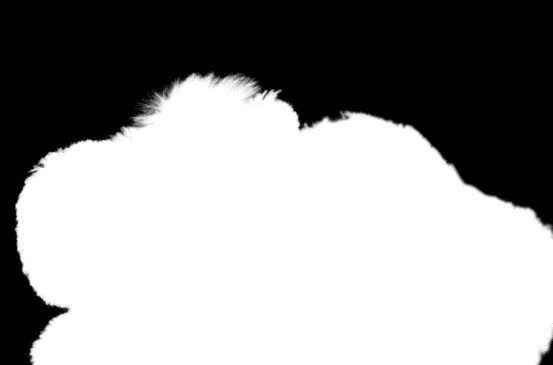
\includegraphics[width=0.4\columnwidth]{Chapter5/5/bear_ours.png}}
\caption[GT012 benchmark image with various results.]{GT012 ground truth in comparison with our result.}
\label{fig:bear-f}
\end{figure}

